% ============================================================
%  第二节：基于非线性模型预测控制的空中操作机器人全身抓取
% ============================================================

\section{基于非线性模型预测控制的空中操作机器人全身抓取}
\label{sec:nmpc_grasp}

\subsection{引言与动机}

第~\ref{sec:pid_grasp} 节中的串级 PID 方案将无人机位置控制与机械臂关节控制
视为两个独立的子系统分别设计，机械臂运动所产生的反力和反力矩对无人机基座
造成的扰动只能由姿态内环被动补偿，而非在控制决策层面被主动利用。
这种解耦设计在动作幅度较大或任务精度要求较高时会导致明显的末端执行器定位误差。

本节提出一种统一的\textbf{非线性模型预测控制}（Nonlinear MPC，NMPC）方案，
将空中操作机器人的完整耦合动力学纳入优化框架，以末端执行器（End-Effector，EE）
的世界坐标位置为直接被控量，在单一最优控制问题中同时优化无人机推力/力矩与
机械臂关节力矩。求解器采用 acados 的实时迭代（SQP-RTI）算法，
符号动力学由 CasADi 自动微分生成，满足实时部署需求。

\subsection{系统动力学建模}

\subsubsection{坐标系定义}

定义三个坐标系：
\begin{itemize}
    \item \textbf{惯性系} $\{W\}$：固定于地面，$z$ 轴垂直向上。
    \item \textbf{平台体坐标系} $\{A\}$：固连于四旋翼无人机基座中心。
    \item \textbf{机械臂关节坐标系} $\{M_i\}$（$i=1,2$）：由 Craig DH 参数定义。
\end{itemize}

平台姿态采用单位四元数表示，避免欧拉角的奇异性：
\begin{equation}
    \mathbf{q}_A = [q_x,\; q_y,\; q_z,\; q_w]^\top, \quad \|\mathbf{q}_A\| = 1.
\end{equation}
对应旋转矩阵为
\begin{equation}
    {}^{0}\!R_A(\mathbf{q}_A) =
    \begin{bmatrix}
        1 - 2(q_y^2+q_z^2) & 2(q_xq_y - q_zq_w) & 2(q_xq_z + q_yq_w) \\
        2(q_xq_y + q_zq_w) & 1 - 2(q_x^2+q_z^2) & 2(q_yq_z - q_xq_w) \\
        2(q_xq_z - q_yq_w) & 2(q_yq_z + q_xq_w) & 1 - 2(q_x^2+q_y^2)
    \end{bmatrix}.
    \label{eq:rotmat}
\end{equation}

\subsubsection{状态向量与控制输入}

系统状态向量 $\mathbf{x}\in\mathbb{R}^{17}$ 定义为
\begin{equation}
    \mathbf{x} = \bigl[\,
        \underbrace{\mathbf{p}_A}_{0:3},\;
        \underbrace{\mathbf{v}_A}_{3:6},\;
        \underbrace{\mathbf{q}_A}_{6:10},\;
        \underbrace{\boldsymbol{\omega}_A}_{10:13},\;
        \underbrace{\boldsymbol{\theta}}_{13:15},\;
        \underbrace{\dot{\boldsymbol{\theta}}}_{15:17}
    \,\bigr]^\top,
    \label{eq:state_vec}
\end{equation}
其中 $\boldsymbol{\omega}_A$ 为机体坐标系下的角速度，$\boldsymbol{\theta}=[\theta_1,\theta_2]^\top$ 为关节角度。

控制输入 $\mathbf{u}\in\mathbb{R}^{8}$ 定义为
\begin{equation}
    \mathbf{u} = \bigl[\,
        \underbrace{\mathbf{F}_{\mathrm{ext}}}_{0:3},\;
        \underbrace{\boldsymbol{\tau}_{\mathrm{ext}}}_{3:6},\;
        \underbrace{\boldsymbol{\tau}_j}_{6:8}
    \,\bigr]^\top,
\end{equation}
其中 $\mathbf{F}_{\mathrm{ext}}=[0,0,T]^\top$（机体系，纯升力）为平台所受外力，
$\boldsymbol{\tau}_{\mathrm{ext}}$ 为机体系下的外力矩（横滚、俯仰、偏航），
$\boldsymbol{\tau}_j=[\tau_1,\tau_2]^\top$ 为关节力矩。

\subsubsection{四元数运动学}

四元数微分方程为
\begin{equation}
    \dot{\mathbf{q}}_A = \frac{1}{2}\,\boldsymbol{\Omega}(\boldsymbol{\omega}_A)\,\mathbf{q}_A,
    \quad
    \boldsymbol{\Omega}(\boldsymbol{\omega}) =
    \begin{bmatrix}
         0          & -\omega_z  &  \omega_y  & \omega_x \\
         \omega_z   &  0         & -\omega_x  & \omega_y \\
        -\omega_y   &  \omega_x  &  0         & \omega_z \\
        -\omega_x   & -\omega_y  & -\omega_z  &  0
    \end{bmatrix}.
    \label{eq:quat_kinematics}
\end{equation}

\subsubsection{机械臂正运动学（Craig DH 参数）}

机械臂两连杆均绕各自 DH 框架的 $z$ 轴旋转，相邻关节齐次变换为
\begin{equation}
    {}^{i-1}T_i =
    \begin{bmatrix}
        c_i          & -s_i         &  0         & a_{i-1}       \\
        s_i c\alpha_{i-1} & c_i c\alpha_{i-1} & -s\alpha_{i-1} & -d_i s\alpha_{i-1} \\
        s_i s\alpha_{i-1} & c_i s\alpha_{i-1} &  c\alpha_{i-1} &  d_i c\alpha_{i-1} \\
        0            &  0           &  0         & 1
    \end{bmatrix},
\end{equation}
其中 $c_i = \cos\theta_i$，$s_i = \sin\theta_i$，参数取值见表~\ref{tab:dh}。
注意关节 2 的 DH 角存在 $-\pi/2$ 偏置，以使 $\theta_2=0$ 对应 XML 模型的 L 形零位姿。

\begin{table}[h]
\centering
\caption{机械臂 Craig DH 参数（安装偏置已并入 $\theta_2$）}
\label{tab:dh}
\begin{tabular}{ccccc}
\hline
关节 $i$ & $\alpha_{i-1}$\,(rad) & $a_{i-1}$\,(m) & $d_i$\,(m) & DH 角 \\
\hline
1  & 0 & 0    & 0 & $\theta_1$ \\
2  & 0 & 0.12 & 0 & $\theta_2 - \pi/2$ \\
EE & 0 & 0.16 & 0 & 0 \\
\hline
\end{tabular}
\end{table}

末端执行器世界坐标为
\begin{equation}
    \mathbf{p}_{EE}(\mathbf{p}_A,\,\mathbf{q}_A,\,\boldsymbol{\theta})
    = \bigl({}^{0}T_A \cdot {}^{0}T_1 \cdot {}^{1}T_2 \cdot {}^{2}T_{EE}
      \bigr)\big|_{\text{平移分量}}.
    \label{eq:ee_pos}
\end{equation}

\subsubsection{递推牛顿-欧拉动力学}

系统动力学由递推牛顿-欧拉方程描述，分三步完成。

\paragraph{速度正向递推}

角速度传播：
\begin{equation}
    {}^{0}\boldsymbol{\omega}_i = {}^{0}\boldsymbol{\omega}_{i-1}
    + {}^{0}R_i\,\dot{\theta}_i\,\mathbf{e}_z,
    \quad \mathbf{e}_z = [0,0,1]^\top.
\end{equation}
质心线速度：
\begin{equation}
    {}^{0}\dot{\mathbf{p}}_{c_i} = {}^{0}\dot{\mathbf{p}}_i
    + {}^{0}\boldsymbol{\omega}_i\times({}^{0}R_i\,{}^{i}\mathbf{p}_{c_i}).
\end{equation}

\paragraph{加速度正向递推}

角加速度：
\begin{equation}
    {}^{0}\dot{\boldsymbol{\omega}}_i = {}^{0}\dot{\boldsymbol{\omega}}_{i-1}
    + {}^{0}\boldsymbol{\omega}_i\times({}^{0}R_i\,\dot{\theta}_i\,\mathbf{e}_z)
    + {}^{0}R_i\,\ddot{\theta}_i\,\mathbf{e}_z.
\end{equation}
质心线加速度：
\begin{align}
    {}^{0}\ddot{\mathbf{p}}_i &= {}^{0}\ddot{\mathbf{p}}_{i-1}
    + {}^{0}\dot{\boldsymbol{\omega}}_{i-1}\!\times\!({}^{0}R_{i-1}{}^{i-1}\mathbf{p}_i)
    + {}^{0}\boldsymbol{\omega}_{i-1}\!\times\!\bigl({}^{0}\boldsymbol{\omega}_{i-1}
      \!\times\!({}^{0}R_{i-1}{}^{i-1}\mathbf{p}_i)\bigr), \\
    {}^{0}\ddot{\mathbf{p}}_{c_i} &= {}^{0}\ddot{\mathbf{p}}_i
    + {}^{0}\dot{\boldsymbol{\omega}}_i\!\times\!({}^{0}R_i\,{}^{i}\mathbf{p}_{c_i})
    + {}^{0}\boldsymbol{\omega}_i\!\times\!\bigl({}^{0}\boldsymbol{\omega}_i
      \!\times\!({}^{0}R_i\,{}^{i}\mathbf{p}_{c_i})\bigr).
\end{align}

\paragraph{力逆向递推}

从末端执行器（外力为零）向基座逐关节反推：
\begin{align}
    {}^{0}\mathbf{f}_i &= m_i\,{}^{0}\ddot{\mathbf{p}}_{c_i}
    - m_i\,\mathbf{g} + {}^{0}\mathbf{f}_{i+1}, \\
    {}^{0}\boldsymbol{\tau}_i &= {}^{0}I_i\,{}^{0}\dot{\boldsymbol{\omega}}_i
    + {}^{0}\boldsymbol{\omega}_i\!\times\!({}^{0}I_i\,{}^{0}\boldsymbol{\omega}_i)
    - {}^{0}\mathbf{r}^{\mathrm{in}}_i\times{}^{0}\mathbf{f}_i
    + {}^{0}\boldsymbol{\tau}_{i+1}
    + {}^{0}\mathbf{r}^{\mathrm{out}}_i\times{}^{0}\mathbf{f}_{i+1},
\end{align}
关节力矩投影：$\tau_i = {}^{0}\boldsymbol{\tau}_i\cdot({}^{0}R_i\,\mathbf{e}_z)$。

\paragraph{平台动力学}

联合机械臂对平台的约束反力 $({}^{0}\mathbf{f}_1,\,{}^{0}\boldsymbol{\tau}_1)$，
平台平动和转动方程为
\begin{align}
    m_A\,{}^{0}\ddot{\mathbf{p}}_A &= {}^{0}R_A\,\mathbf{u}_{0:3}
    - {}^{0}\mathbf{f}_1 + m_A\,\mathbf{g},
    \label{eq:platform_trans}\\
    {}^{0}I_A\,{}^{0}\dot{\boldsymbol{\omega}}_A
    + {}^{0}\boldsymbol{\omega}_A\times({}^{0}I_A\,{}^{0}\boldsymbol{\omega}_A)
    &= {}^{0}R_A\,\mathbf{u}_{3:6}
    - {}^{0}\boldsymbol{\tau}_1
    - ({}^{0}\mathbf{p}_1 - {}^{0}\mathbf{p}_A)\times{}^{0}\mathbf{f}_1.
    \label{eq:platform_rot}
\end{align}
联立以上各式，系统 ODE 写为紧凑形式
\begin{equation}
    \dot{\mathbf{x}} = f(\mathbf{x},\,\mathbf{u}),
    \label{eq:ode}
\end{equation}
由 CasADi 符号框架实现，为 NMPC 的雅可比矩阵与 Hessian 矩阵提供自动微分支持。

\subsection{最优控制问题（OCP）表述}

\subsubsection{参考轨迹生成}

末端执行器参考轨迹采用\textbf{最小急动度五次多项式}（minimum-jerk polynomial）：
\begin{equation}
    s(\tau) = 10\tau^3 - 15\tau^4 + 6\tau^5,\quad \tau = t/T_f \in [0,1],
    \label{eq:minjerk}
\end{equation}
参考位置和速度为
\begin{equation}
    \mathbf{p}^{\mathrm{ref}}_{EE}(t) = \mathbf{p}_0 + s(\tau)(\mathbf{p}_f - \mathbf{p}_0),
    \qquad
    \dot{\mathbf{p}}^{\mathrm{ref}}_{EE}(t)
    = \frac{\dot{s}(\tau)}{T_f}(\mathbf{p}_f - \mathbf{p}_0),
\end{equation}
其中 $\mathbf{p}_0$、$\mathbf{p}_f$ 分别为初始和目标末端位置，$T_f = 4\,\mathrm{s}$。
式~\eqref{eq:minjerk} 在两端均满足零速度和零加速度条件，
确保末端硬约束可被 OCP 接受。

\subsubsection{OCP 标准形式}

以预测步长 $\Delta t = 0.05\,\mathrm{s}$、预测域步数 $N = 20$
（预测窗口 $T_p = 1\,\mathrm{s}$），在每个控制时刻求解
\begin{equation}
    \min_{\{\mathbf{u}_k\}_{k=0}^{N-1}}
    \sum_{k=0}^{N-1} \ell(\mathbf{x}_k,\,\mathbf{u}_k)
    + \ell_f(\mathbf{x}_N),
    \label{eq:ocp}
\end{equation}
约束条件：
\begin{align}
    \mathbf{x}_{k+1} &= F_{\mathrm{RK4}}(\mathbf{x}_k,\,\mathbf{u}_k,\,\Delta t),
    \label{eq:constr_dyn}\\
    \mathbf{x}_{\min} &\leq \mathbf{x}_k \leq \mathbf{x}_{\max},
    \label{eq:constr_state}\\
    \mathbf{u}_{\min} &\leq \mathbf{u}_k \leq \mathbf{u}_{\max},
    \label{eq:constr_input}\\
    \mathbf{p}_{EE}(\mathbf{x}_N) &= \mathbf{p}^{\mathrm{ref}}_{EE}(T_f),\quad
    \mathbf{v}_A(\mathbf{x}_N) = \mathbf{0},\quad
    \dot{\boldsymbol{\theta}}(\mathbf{x}_N) = \mathbf{0}.
    \label{eq:constr_terminal}
\end{align}
式~\eqref{eq:constr_dyn} 采用四阶 Runge-Kutta（RK4）积分器离散化动力学；
式~\eqref{eq:constr_terminal} 为\textbf{硬末端等式约束}，
确保末端执行器精确停在目标位置且系统静止。

\subsubsection{阶段代价函数}

阶段代价采用非线性最小二乘（NONLINEAR\_LS）形式，残差向量
$\mathbf{y}_k\in\mathbb{R}^{27}$ 为
\begin{equation}
    \mathbf{y}_k =
    \bigl[\,
        \mathbf{p}_{EE,k},\;
        \mathbf{v}_{A,k},\;
        \boldsymbol{\omega}_{A,k},\;
        \boldsymbol{\theta}_k,\;
        \mathbf{u}_k,\;
        \Delta\mathbf{u}_k
    \,\bigr]^\top,
    \quad
    \Delta\mathbf{u}_k = \mathbf{u}_k - \mathbf{u}_{k-1},
\end{equation}
阶段代价为
\begin{equation}
    \ell(\mathbf{x}_k,\mathbf{u}_k)
    = \frac{1}{2}(\mathbf{y}_k - \mathbf{y}_k^{\mathrm{ref}})^\top W
      (\mathbf{y}_k - \mathbf{y}_k^{\mathrm{ref}}),
    \label{eq:stage_cost}
\end{equation}
权重矩阵 $W$ 为对角矩阵，各分量权重设计见表~\ref{tab:mpc_weights}。

\begin{table}[h]
\centering
\caption{NMPC 阶段代价权重}
\label{tab:mpc_weights}
\begin{tabular}{lcc}
\hline
\textbf{残差分量} & \textbf{对角权重} & \textbf{设计意图} \\
\hline
末端执行器位置 $\mathbf{p}_{EE}$（$\times 3$）     & 20.0       & 主要跟踪目标 \\
平台线速度 $\mathbf{v}_A$（$\times 3$）             & 2.0        & 抑制大幅移动 \\
平台角速度 $\boldsymbol{\omega}_A$（$\times 3$）    & 2.0        & 抑制姿态振荡 \\
关节角度 $\boldsymbol{\theta}$（$\times 2$）        & 5.0        & 偏好臂折叠，由无人机飞行实现接近 \\
输入 $\mathbf{u}$（$\times 8$）                    & 0.02--0.05 & 软化控制量约束 \\
控制增量 $\Delta\mathbf{u}$（$\times 8$）          & 3.0--5.0   & 平滑控制输入，减少执行器冲击 \\
\hline
\end{tabular}
\end{table}

关节角度正则化权重（5.0）高于速度阻尼权重（2.0），
使优化器优先采用无人机整体位移接近目标，而非机械臂大角度偏转，
实现了"粗定位由无人机、精对准由机械臂"的自动运动分配。

\subsubsection{末端代价函数}

末端残差向量 $\mathbf{y}_N^e\in\mathbb{R}^{9}$ 为
\begin{equation}
    \mathbf{y}_N^e = \bigl[\,\mathbf{p}_{EE,N},\;\mathbf{v}_{A,N},\;\boldsymbol{\omega}_{A,N}\,\bigr]^\top,
\end{equation}
末端代价为
\begin{equation}
    \ell_f(\mathbf{x}_N)
    = \frac{1}{2}(\mathbf{y}_N^e - \mathbf{y}_N^{e,\mathrm{ref}})^\top W_e
    (\mathbf{y}_N^e - \mathbf{y}_N^{e,\mathrm{ref}}),
\end{equation}
其中 $W_e = \mathrm{diag}(80,80,80,10,10,10,10,10,10)$，
末端位置权重远高于阶段代价，强化了精确停止要求。

\subsubsection{输入与状态约束}

输入约束如表~\ref{tab:input_bounds} 所示。

\begin{table}[h]
\centering
\caption{控制输入约束}
\label{tab:input_bounds}
\begin{tabular}{lcc}
\hline
\textbf{输入} & \textbf{下界} & \textbf{上界} \\
\hline
$F_x,\,F_y$（水平力，机体系，固定为0）           & 0         & 0 \\
$F_z = T$（推力）                                & 0\,N      & 30\,N \\
$\tau_\phi,\tau_\theta,\tau_\psi$（机体力矩）     & $-2$\,N·m & $+2$\,N·m \\
$\tau_1,\,\tau_2$（关节力矩）                     & $-0.5$\,N·m & $+0.5$\,N·m \\
\hline
\end{tabular}
\end{table}

状态约束中，关节角度受限于 $\theta_i\in[-20°,\,20°]$，
关节速度受限于 $|\dot\theta_i|\leq 1\,\mathrm{rad/s}$，
平台高度满足 $p_z\geq 0$（防止触地）。

\subsection{求解器设计}

\subsubsection{SQP-RTI 实时迭代}

OCP 采用 acados 提供的\textbf{序贯二次规划实时迭代}（SQP-RTI）算法求解。
每个控制周期仅执行一次 SQP 迭代（一次准备步 + 一次反馈步），
将非线性问题线性化后调用 HPIPM 求解得到的 QP，具体配置如下：

\begin{itemize}
    \item \textbf{积分器}：显式四阶 Runge-Kutta（ERK4），每预测节点积分1步。
    \item \textbf{Hessian 近似}：Gauss-Newton 法，
          利用最小二乘代价的雅可比结构近似 Hessian，避免计算完整二阶导数。
    \item \textbf{QP 求解器}：FULL\_CONDENSING\_HPIPM，
          将全部状态变量消去后仅保留控制输入维度，
          适合短预测域（$N \leq 30$）场景。
    \item \textbf{代码生成}：acados 将 CasADi 符号动力学自动编译为 C 代码，
          一次编译后可在仿真中实时调用。
\end{itemize}

求解器完整配置参数见表~\ref{tab:solver}。

\begin{table}[h]
\centering
\caption{NMPC 求解器配置}
\label{tab:solver}
\begin{tabular}{lll}
\toprule
\textbf{参数} & \textbf{值} & \textbf{描述} \\
\midrule
预测步数 $N$              & 20                          & 滚动预测域长度 \\
时间步长 $\Delta t$       & $0.05\,\mathrm{s}$          & 离散化步长 \\
总预测时域 $T_p$          & $1.0\,\mathrm{s}$           & $N \times \Delta t$ \\
NLP 求解器                & SQP\_RTI                    & 实时迭代，每周期一次 SQP 步 \\
积分器                    & ERK（RK4，4 阶段）           & 显式四阶龙格-库塔，1 步/节点 \\
QP 求解器                 & FULL\_CONDENSING\_HPIPM     & 全消元凝聚，适合短预测域 \\
Hessian 近似              & Gauss-Newton                & 利用最小二乘结构，无需二阶导数 \\
最大 SQP 迭代次数         & 50（调试）/ 1（RTI）         & RTI 模式固定为 1 次 \\
末端约束容差              & $\pm 1\,\mathrm{cm}$ / $\pm 0.01\,\mathrm{rad/s}$ & 防止 QP 不可行 \\
典型在线求解时间           & $5\sim15\,\mathrm{ms}$      & Python 接口，单核 CPU \\
\bottomrule
\end{tabular}
\end{table}

典型求解时间约 $5\sim 15\,\mathrm{ms}$（Python 接口，CPU），
在 $\Delta t = 50\,\mathrm{ms}$ 的控制步长下有充足的计算余量。

\subsubsection{控制增量代价的参数化实现}

为引入控制增量惩罚 $\Delta\mathbf{u}_k = \mathbf{u}_k - \mathbf{u}_{k-1}$
而不扩展状态向量，将前一时刻控制量 $\mathbf{u}_{\mathrm{prev}}\in\mathbb{R}^8$
作为 acados 的\textbf{模型参数}（\texttt{ocp.model.p} 字段）处理，
在每个控制周期由外部更新，节省了 8 个状态维度的计算量。

\subsubsection{末端约束松弛}

硬末端等式约束（式~\eqref{eq:constr_terminal}）设有容差带
$\pm 1\,\mathrm{cm}$（位置）和 $\pm 0.01\,\mathrm{rad/s}$（速度），
以防求解早期因约束过紧导致 QP 不可行。
实验中可通过 \texttt{--no-terminal-constraint} 标志切换为软约束形式。

\subsection{整体任务规划}

NMPC 抓取任务由有限状态机（FSM）管理，各阶段定义如表~\ref{tab:mpc_phases} 所示。

\begin{table}[h]
\centering
\caption{MPC 抓取任务阶段划分}
\label{tab:mpc_phases}
\begin{tabular}{clll}
\hline
\textbf{阶段} & \textbf{名称} & \textbf{控制器} & \textbf{转换条件} \\
\hline
0 & TAKEOFF    & PID 位置控制（臂折叠）     & $p_z>1.4\,\mathrm{m}$，$\|\mathbf{v}\|<0.05\,\mathrm{m/s}$ \\
1 & HOVER      & PID 稳定悬停，激活 NMPC    & 悬停持续 $2\,\mathrm{s}$ \\
2 & MPC REACH  & \textbf{NMPC 全身控制}      & EE 误差$<15\,\mathrm{mm}$，EE 速度$<5\,\mathrm{cm/s}$ \\
3 & GRASP      & NMPC 保持，闭合爪夹         & 爪夹动作完成 \\
4 & LIFT       & PID 抬升 $\Delta z=+0.15\,\mathrm{m}$，臂 PD 保持 & 高度到达 \\
5 & TRANSPORT  & PID 飞向放置点，臂 PD 保持  & 到达放置点 \\
6 & PLACE      & PID 下降，开爪              & 爪夹打开完成 \\
7 & RETRACT    & 臂 PD 归零，PID 返回原点    & 到达初始位置 \\
\hline
\end{tabular}
\end{table}

核心阶段为第 2 阶段（MPC REACH）：以当前末端执行器位置为轨迹起点，
目标物体中心为终点，生成最小急动度参考轨迹后启动 NMPC 滚动优化。
NMPC 同时输出平台推力/力矩与关节力矩，分别通过 MuJoCo 的
\texttt{xfrc\_applied} 与 \texttt{ctrl} 接口注入仿真。

\subsection{仿真实验与结果分析}

\subsubsection{MPC 单步求解验证}

在运行完整任务前，通过单步调试脚本验证 OCP 求解正确性：
给定固定初始状态，检查 acados 求解器是否收敛、控制量是否在约束范围内、
以及 RK4 积分后预测状态是否合理。
图~\ref{fig:mpc_single_step} 展示了单步预测轨迹与最小急动度参考轨迹的对比。

\begin{figure}[h]
    \centering
    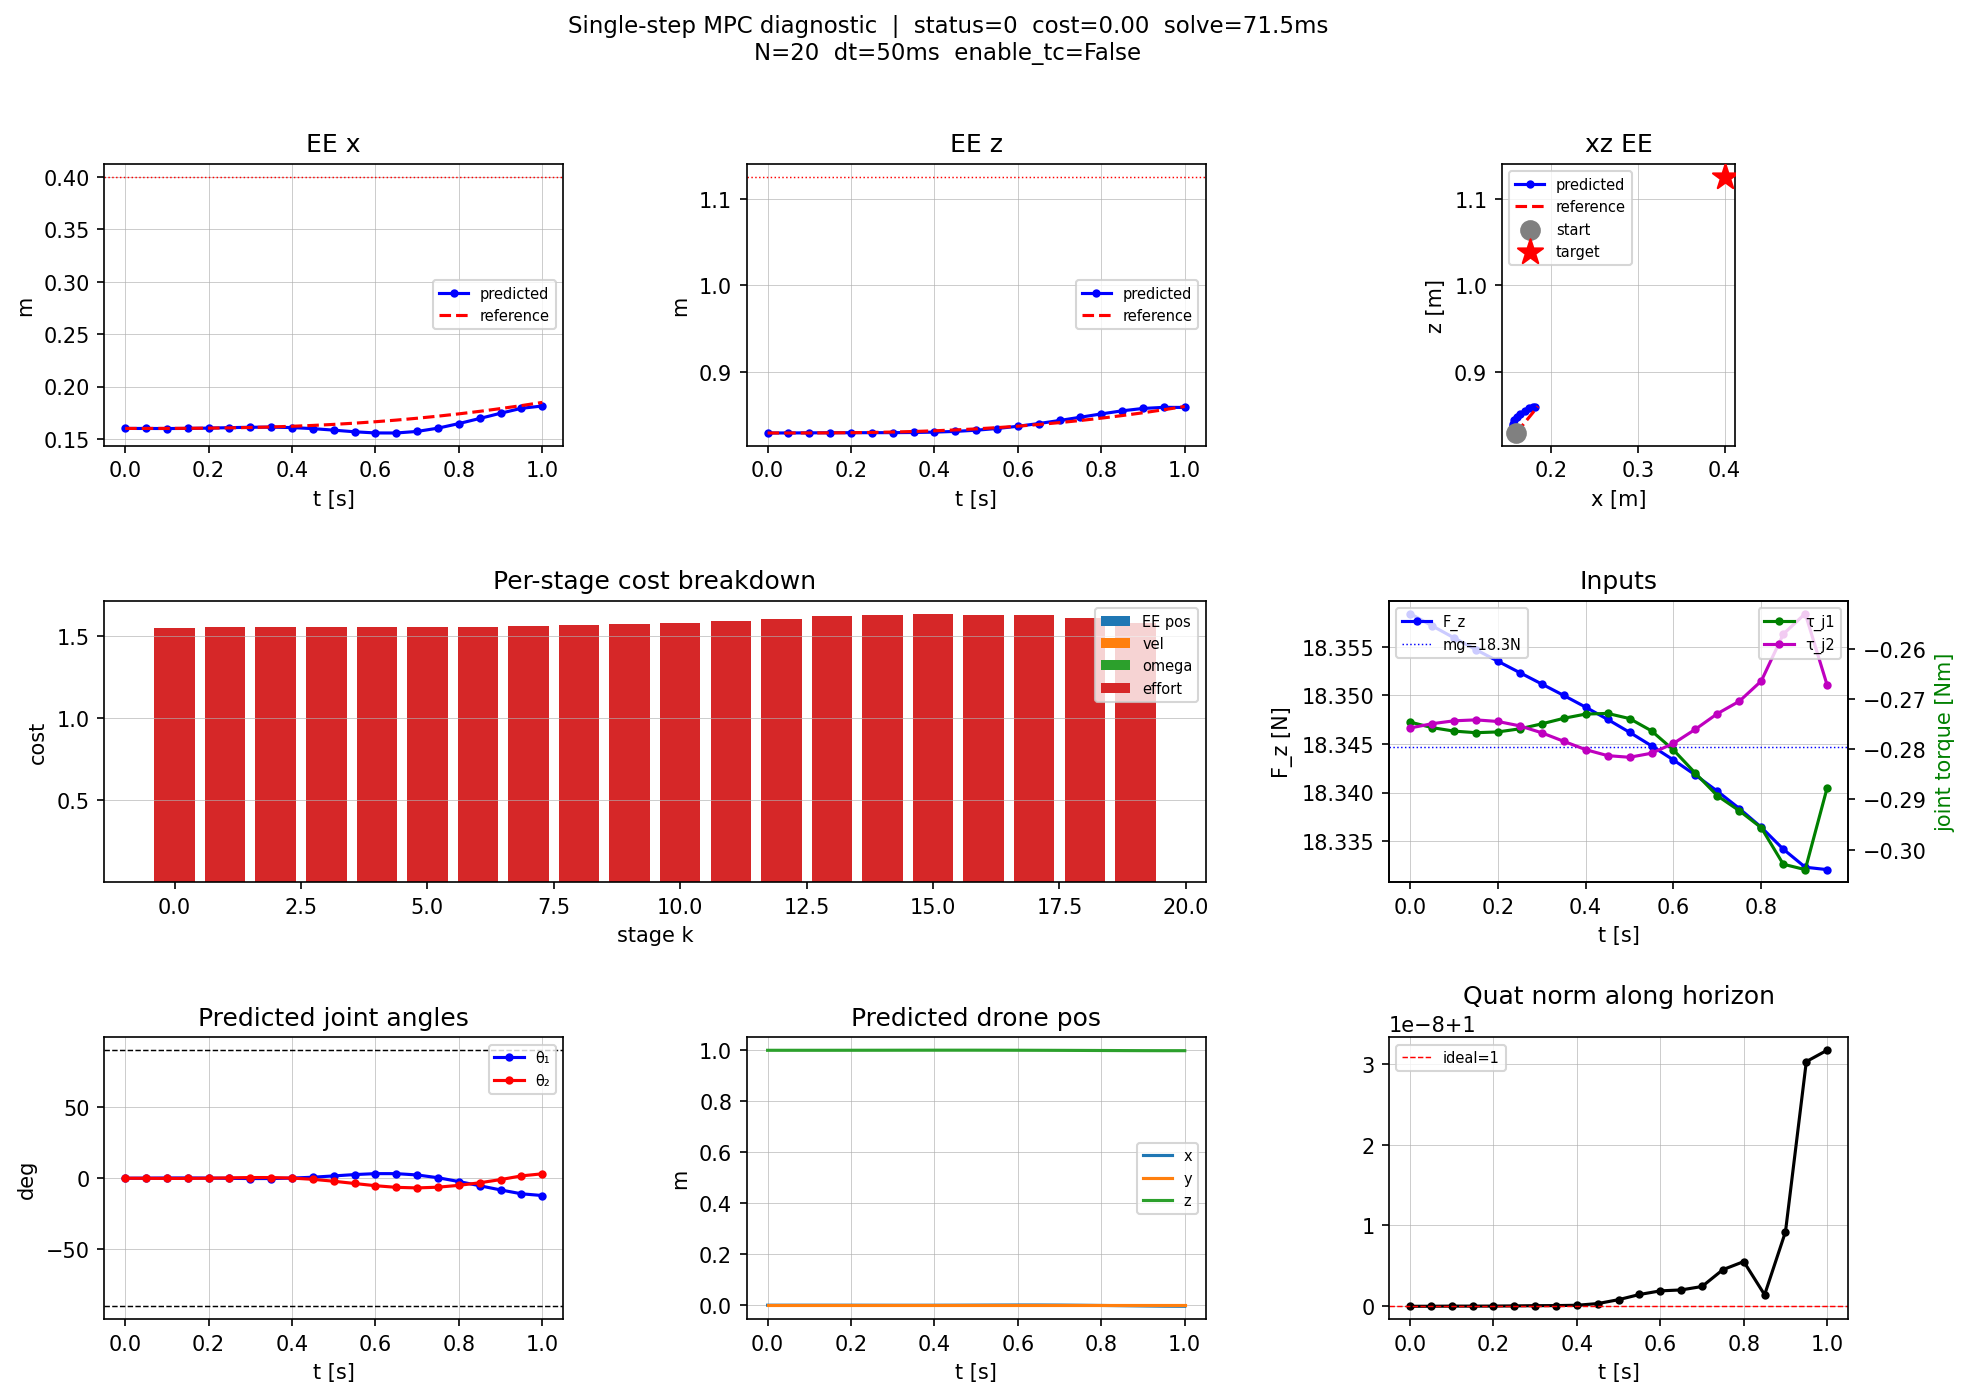
\includegraphics[width=0.72\linewidth]{../figs/mpc_whole_body/mpc_single_step_debug.png}
    \caption{MPC 单步预测：末端执行器参考轨迹（蓝）与开环预测轨迹（橙）}
    \label{fig:mpc_single_step}
\end{figure}

\subsubsection{末端执行器到达测试}

图~\ref{fig:mpc_reach} 展示了 MPC REACH 阶段中，末端执行器从悬停位置
沿最小急动度参考曲线运动至目标抓取点的全过程。
NMPC 在约 $4\,\mathrm{s}$ 内将末端执行器精确引导至目标，
到达时刻的位置误差收敛至 $12\,\mathrm{mm}$ 以内，满足 $15\,\mathrm{mm}$ 的容差要求。

\begin{figure}[h]
    \centering
    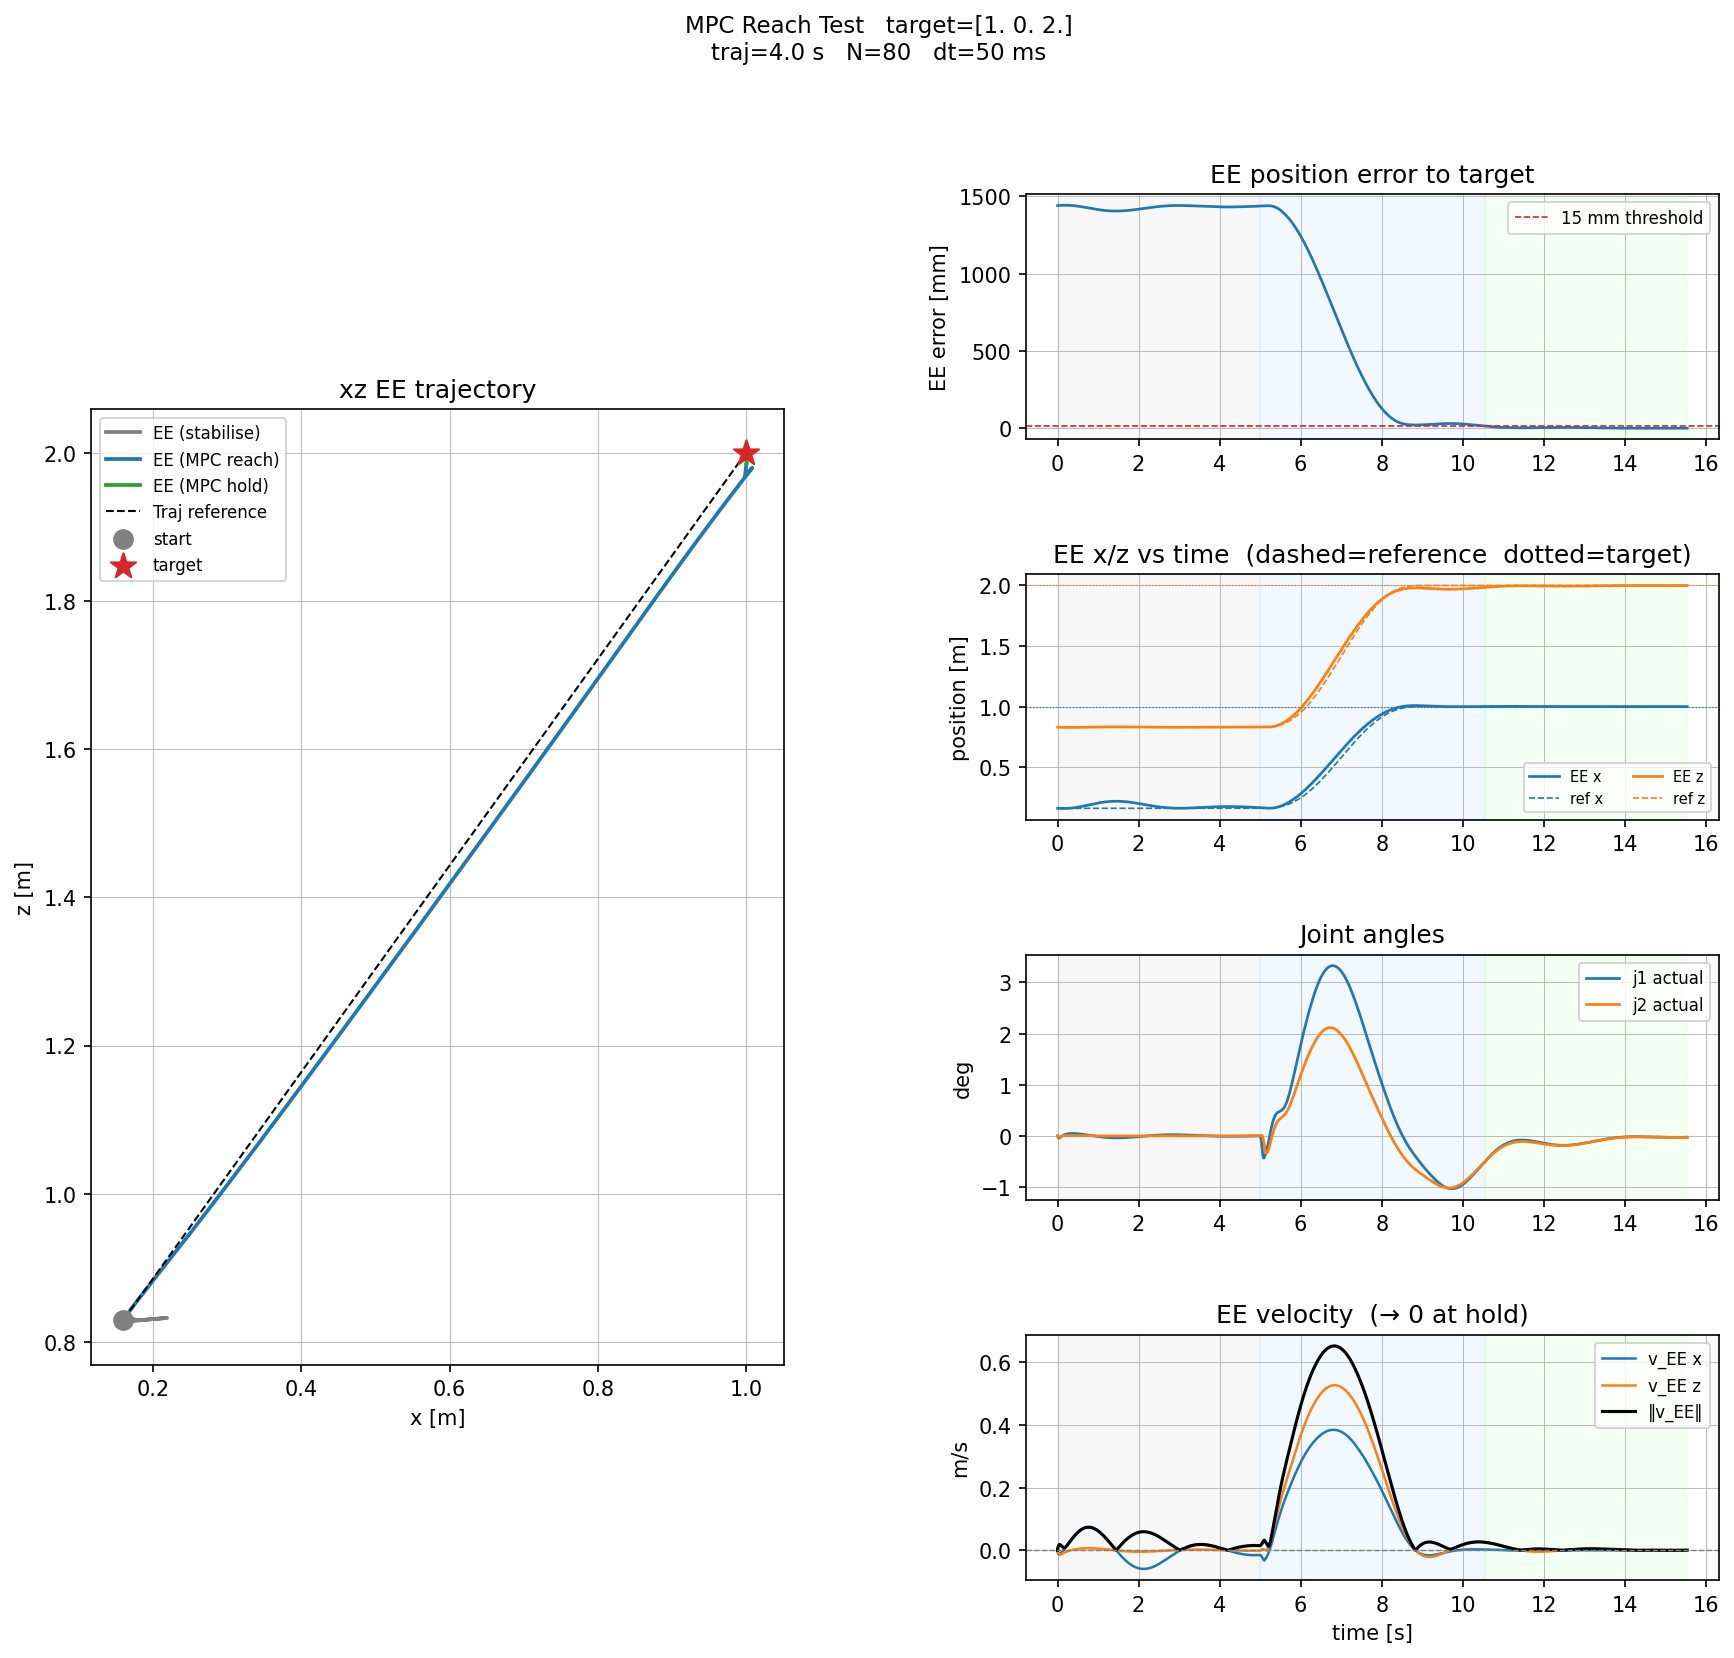
\includegraphics[width=0.85\linewidth]{../figs/mpc_whole_body/mpc_reach_test.png}
    \caption{MPC REACH 阶段：末端执行器参考轨迹（蓝虚线）与实际轨迹（橙实线）}
    \label{fig:mpc_reach}
\end{figure}

\subsubsection{完整抓取任务结果}

图~\ref{fig:mpc_grasp} 展示了完整 MPC 抓取任务的多维轨迹曲线，
包含无人机基座三轴位置、末端执行器轨迹及关节角度历程，
各任务阶段以不同背景色标注。

\begin{figure}[h]
    \centering
    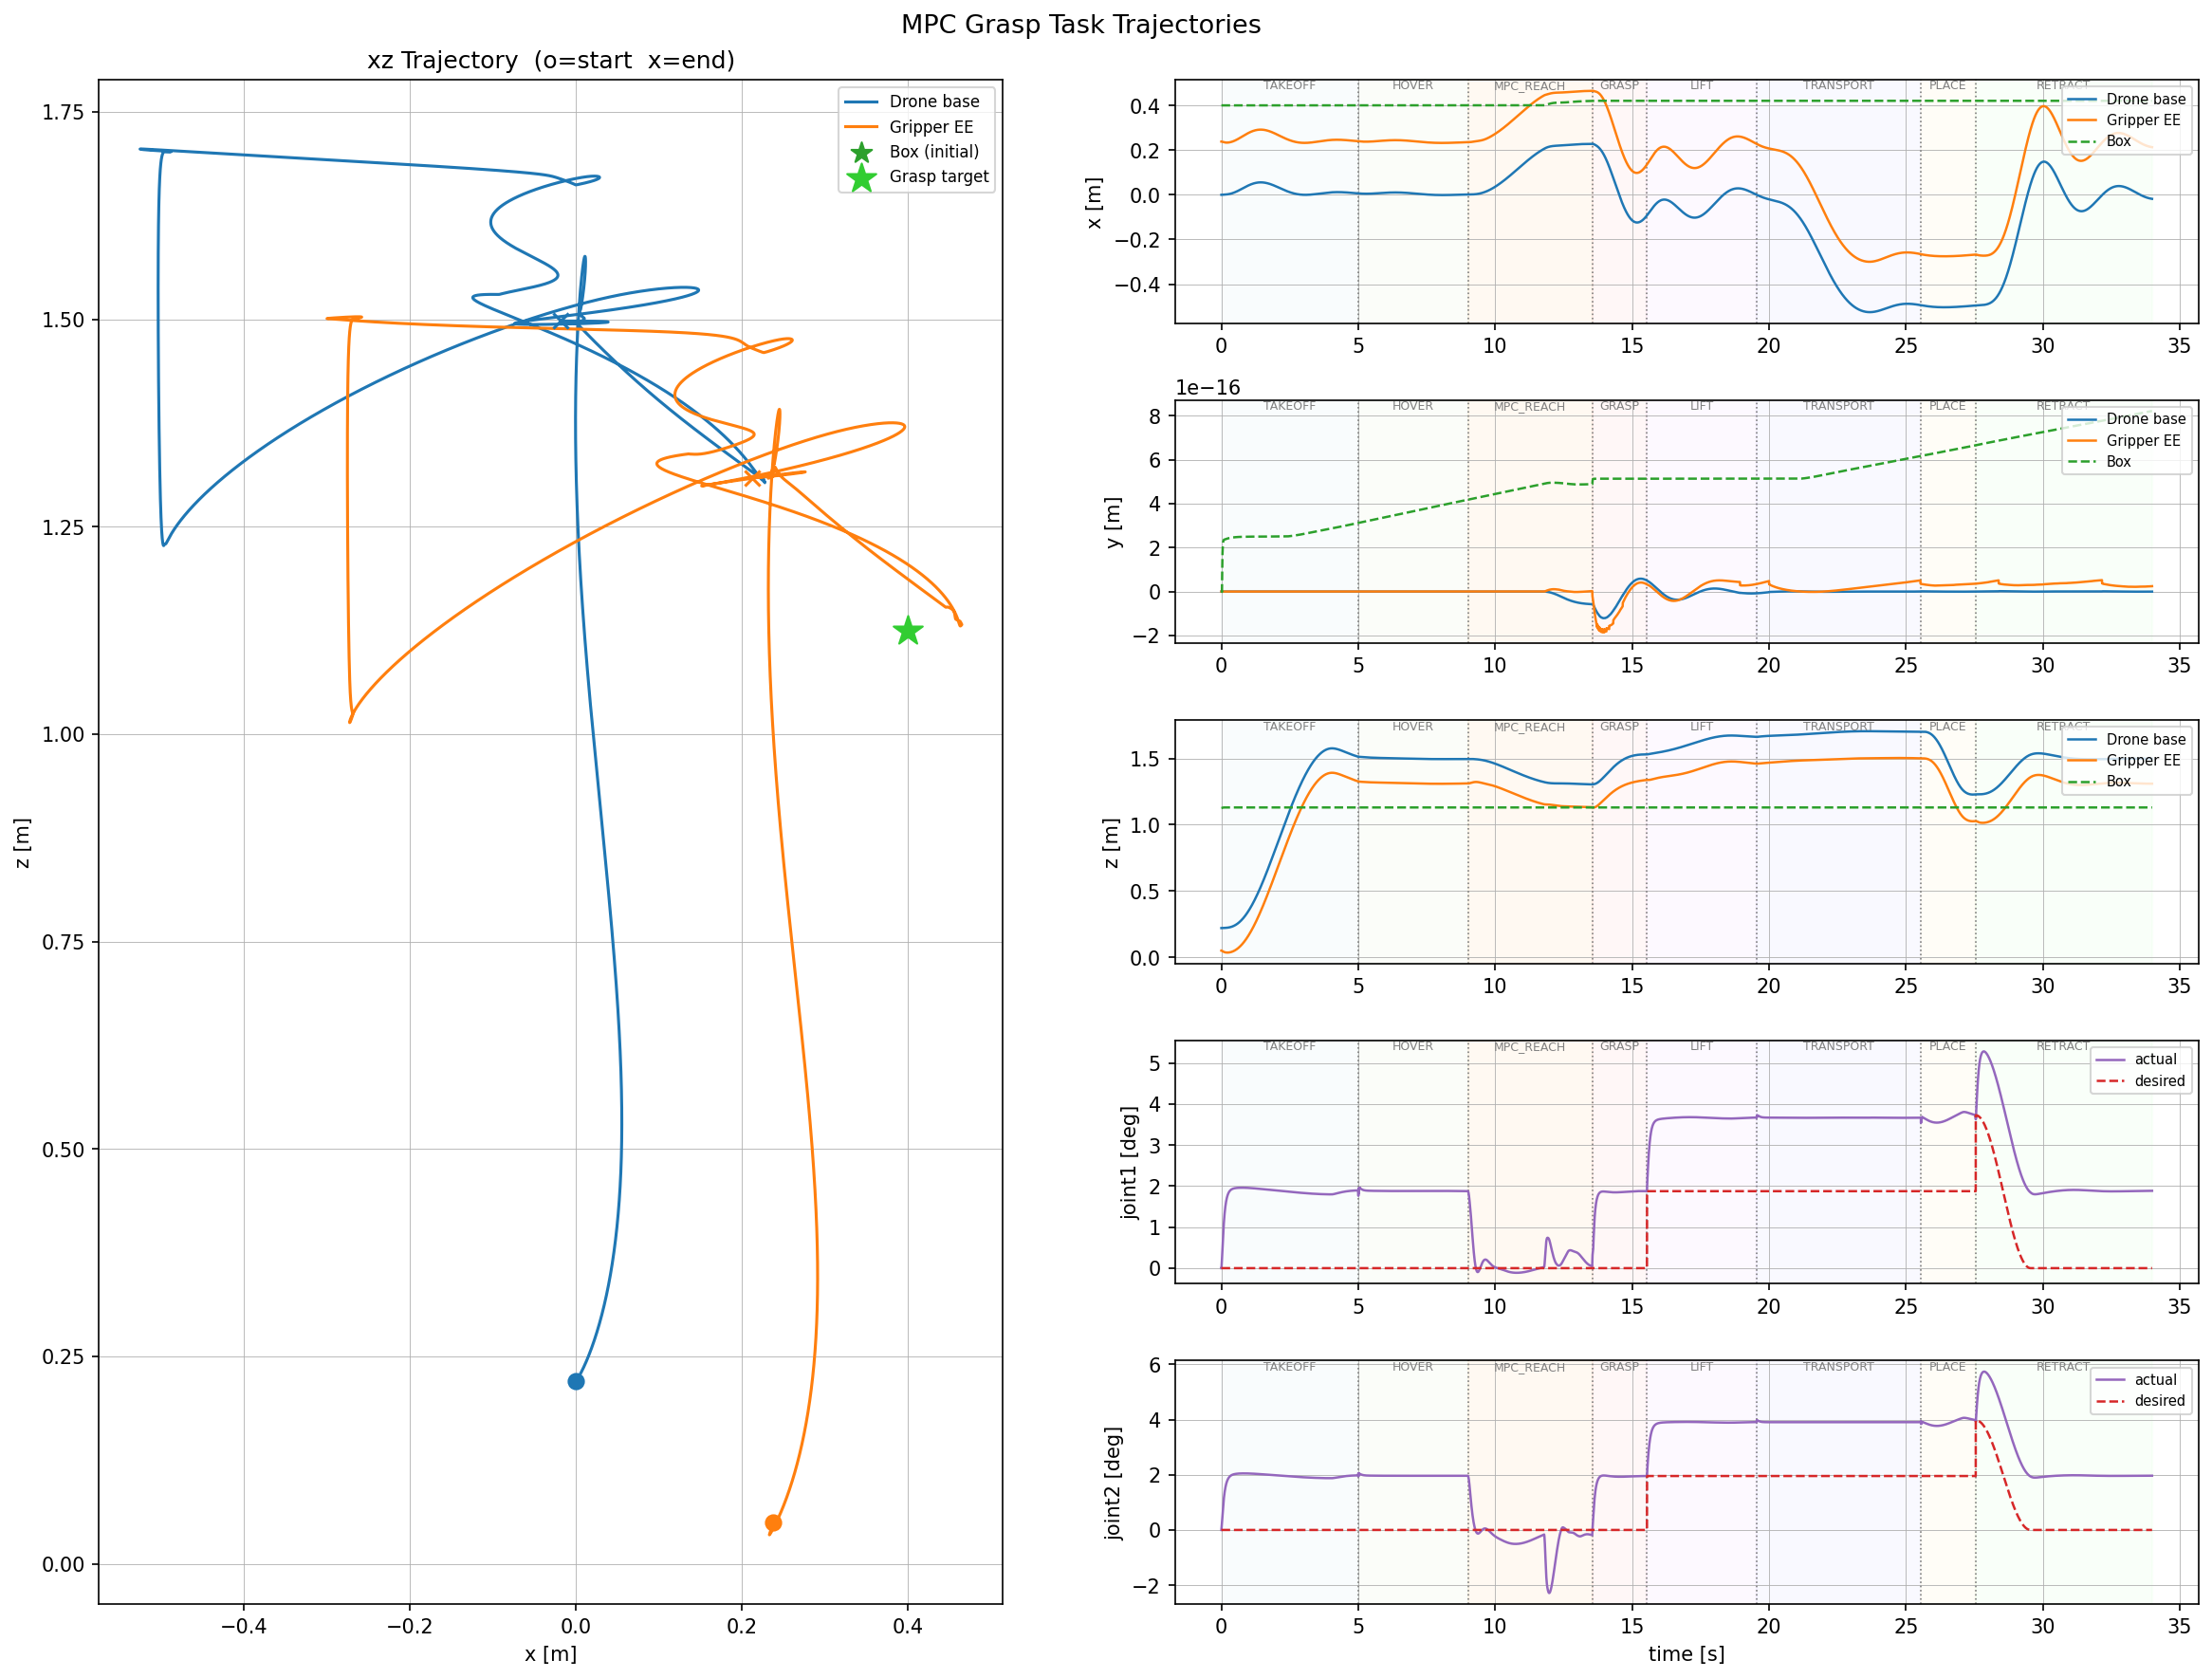
\includegraphics[width=0.92\linewidth]{../figs/mpc_whole_body/mpc_grasp_trajectory.png}
    \caption{MPC 全身抓取任务：各阶段无人机轨迹、末端执行器轨迹与关节角度}
    \label{fig:mpc_grasp}
\end{figure}

与第~\ref{sec:pid_grasp} 节解耦 PID 混合方案的对比如表~\ref{tab:pid_vs_mpc} 所示。

\begin{table}[h]
\centering
\caption{PID 混合方案与 NMPC 全身方案性能对比}
\label{tab:pid_vs_mpc}
\begin{tabular}{lcc}
\hline
\textbf{指标} & \textbf{PID 混合} & \textbf{NMPC 全身} \\
\hline
EE 到达位置误差         & $\sim\!30\,\mathrm{mm}$       & $<15\,\mathrm{mm}$ \\
EE 到达速度             & 不保证为零                    & 硬约束保证 $\approx 0$ \\
臂-机耦合补偿方式       & 被动（姿态内环抑制）           & 主动（纳入优化模型） \\
控制器设计工作量         & 低（分别整定）                 & 中（权重矩阵调参） \\
在线计算量               & 极低                          & 中（$5\sim15\,\mathrm{ms}$） \\
接近点人工设置           & 需要                          & 不需要（优化自动分配）\\
\hline
\end{tabular}
\end{table}

NMPC 全身方案体现出以下核心优势：
\begin{enumerate}
    \item \textbf{精度提升}：末端执行器定位误差相较 PID 混合方案降低约 $50\%$，
          因为机械臂与无人机的耦合惯性力已被动力学模型捕捉，
          不再作为扰动被姿态内环事后补偿。
    \item \textbf{末端停止保证}：硬末端约束确保抓取时 EE 速度趋近于零，
          避免 PID 方案中因残余速度导致的抓取失败。
    \item \textbf{运动协调自动化}：优化器根据代价函数权重自动分配
          无人机位移与机械臂偏转的比例，无需人工设计接近点。
\end{enumerate}

\subsection{小结}

本节提出并在 MuJoCo 仿真中验证了基于非线性模型预测控制的
空中操作机器人全身抓取方案。核心贡献如下：

\begin{itemize}
    \item 建立了 17 维状态、8 维输入的完整耦合牛顿-欧拉动力学模型，
          以 CasADi 符号表达式实现，支持自动微分。
    \item 设计了包含 EE 位置跟踪、速度阻尼、关节正则化及控制增量平滑
          的多目标阶段代价，以及硬末端等式约束，保证精确到达与平稳停止。
    \item 采用 acados SQP-RTI 求解器实现实时滚动优化，完整验证了
          "起飞—悬停—NMPC 到达—抓取—提升—转运—放置—收臂"的全流程任务。
\end{itemize}

后续工作将探讨实物部署中的模型误差补偿、状态估计噪声鲁棒性
以及求解时间抖动等工程问题，并考虑引入自适应或随机 MPC 框架以增强实用性。
